\documentclass{article}
\usepackage{tabularx}
\usepackage{longtable}
\usepackage{array}
\usepackage{float}
\usepackage{listings}
\usepackage{amsmath}
\usepackage{amssymb}
\usepackage{mathtools}
\usepackage{amsfonts}
\usepackage{graphicx}
\usepackage[table]{xcolor}
\setlength{\arrayrulewidth}{0.5mm}
\graphicspath{ {./images} }
\usepackage[margin=20mm]{geometry}
\renewcommand{\labelenumii}{\theenumii}
\renewcommand{\theenumii}{\theenumi.\arabic{enumii}.}
\renewcommand{\arraystretch}{1.5}
\newcommand{\f}[2]{f_{#1}(#2)}
\newcommand{\code}[1]{\texttt{#1}}
\DeclarePairedDelimiter{\ceil}{\lceil}{\rceil}
\DeclarePairedDelimiter{\set}{\left\{}{\right\}}
\DeclarePairedDelimiter{\parens}{\lparen}{\rparen}
\title{HW2 Report}
\date{}
\begin{document}
\maketitle
\section*{Q2:}
    \begin{figure}[H]
        \centering
        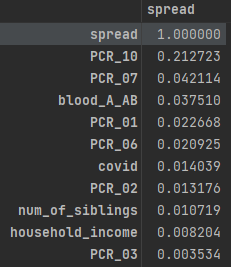
\includegraphics{images/q2.png}
        \caption{The 10 most correlated features to \code{spread}}
    \end{figure}
\section*{Q3:}
    \begin{figure}[H]
        \centering
        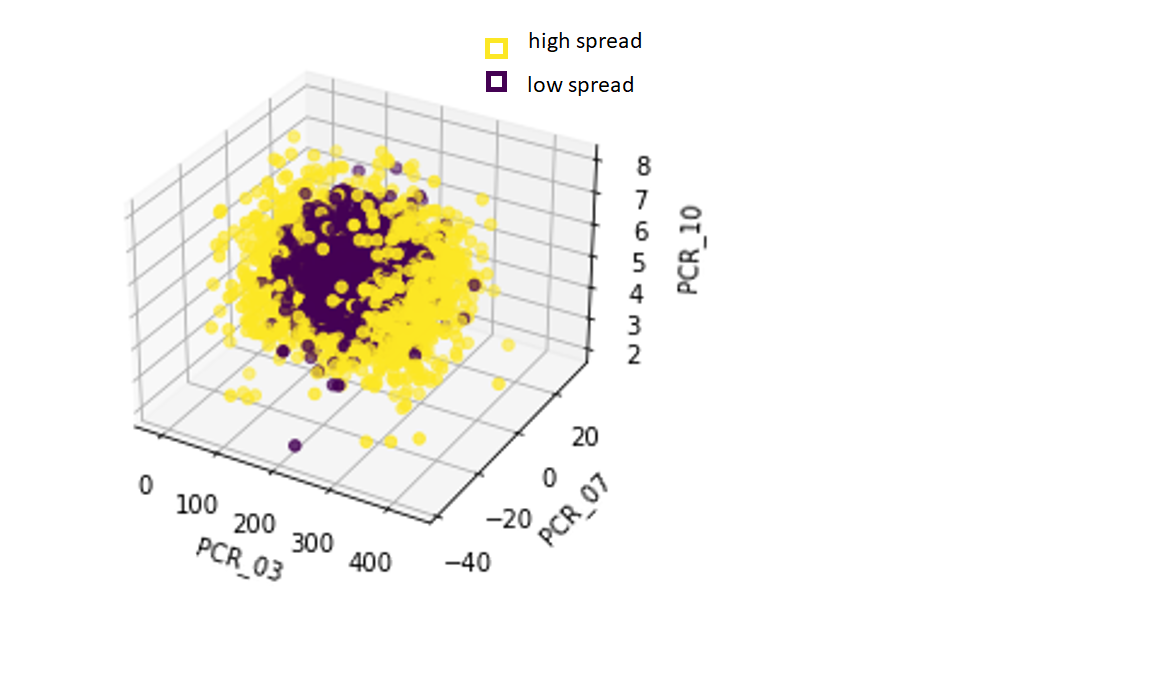
\includegraphics{images/q3.png}
        \caption{3D Scatter plot of \code{PCR\_03}, \code{PCR\_07}, and \code{PCR\_10} according to \code{spread}}
    \end{figure}
\end{document}